\section{Supplementary Note 4: \rev{AI Assisted Corrections and Annotations on MIMIC-III Corpus}}
\rev{We showcase a variety of cases from poor annotations from the original dataset in Fig. \ref{fig:ex_annotation} and our own error analysis of the 4th dataset refinement step in RDMA in Fig. \ref{fig:annotator_agreement_qualitative}.}

\begin{figure}[h]
    \centering
    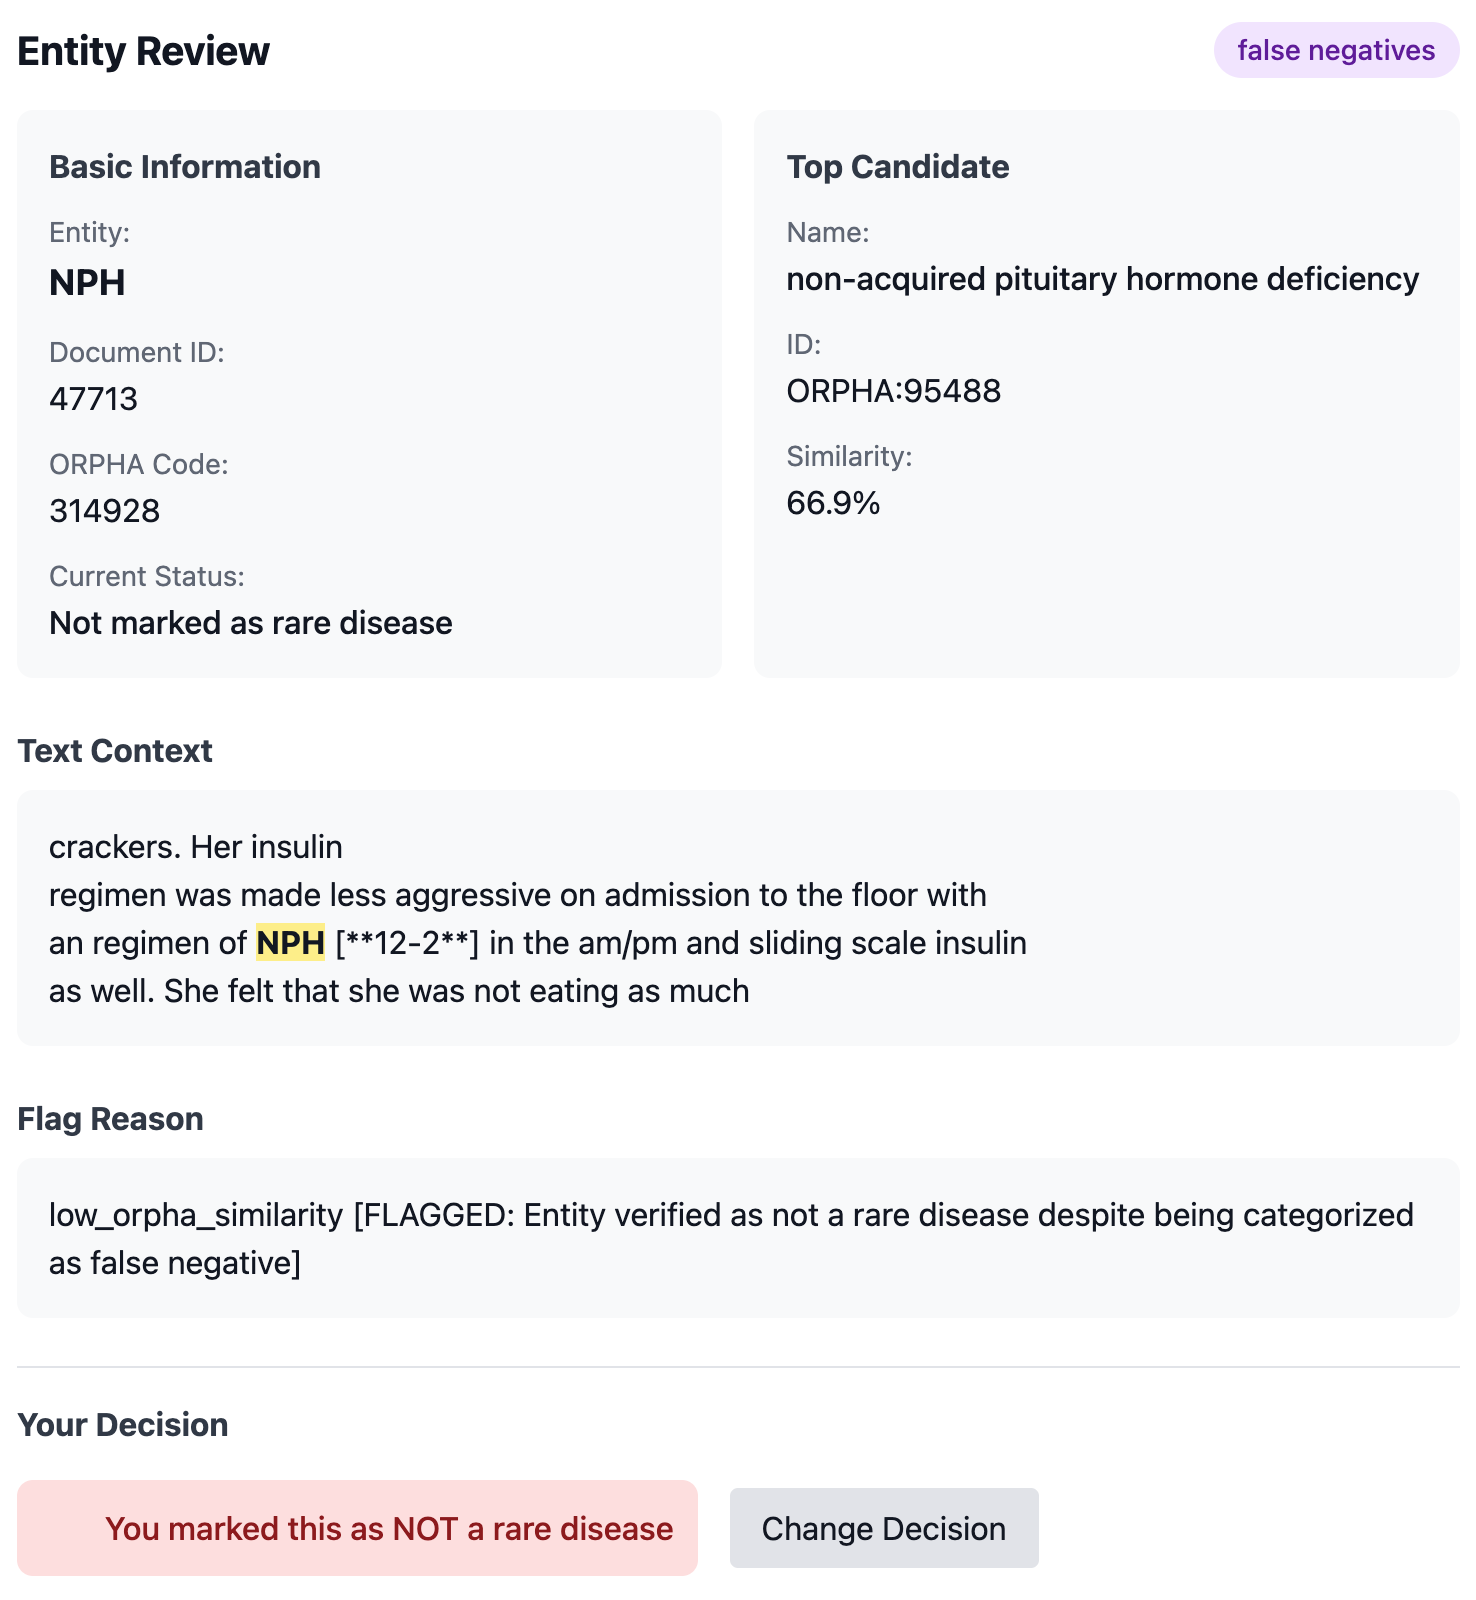
\includegraphics[width=0.55\textwidth]{figs/AnnotationUI.png}
    \caption{\textbf{Example of Inappropriate Annotation in Noisy Dataset.} We note that while NPH as an abbreivation can be related to ``normal pressure hydrocephalus" or other related conditions in the Orphanet ontology as annotated by \cite{dong2023ontology_poor_annotations}, NPH here in this context is actually referring to neutral protamine hagedorn, a type of insulin used to treat diabetes. }
    \label{fig:ex_annotation}
\end{figure}


\begin{figure}[h]
    \centering
    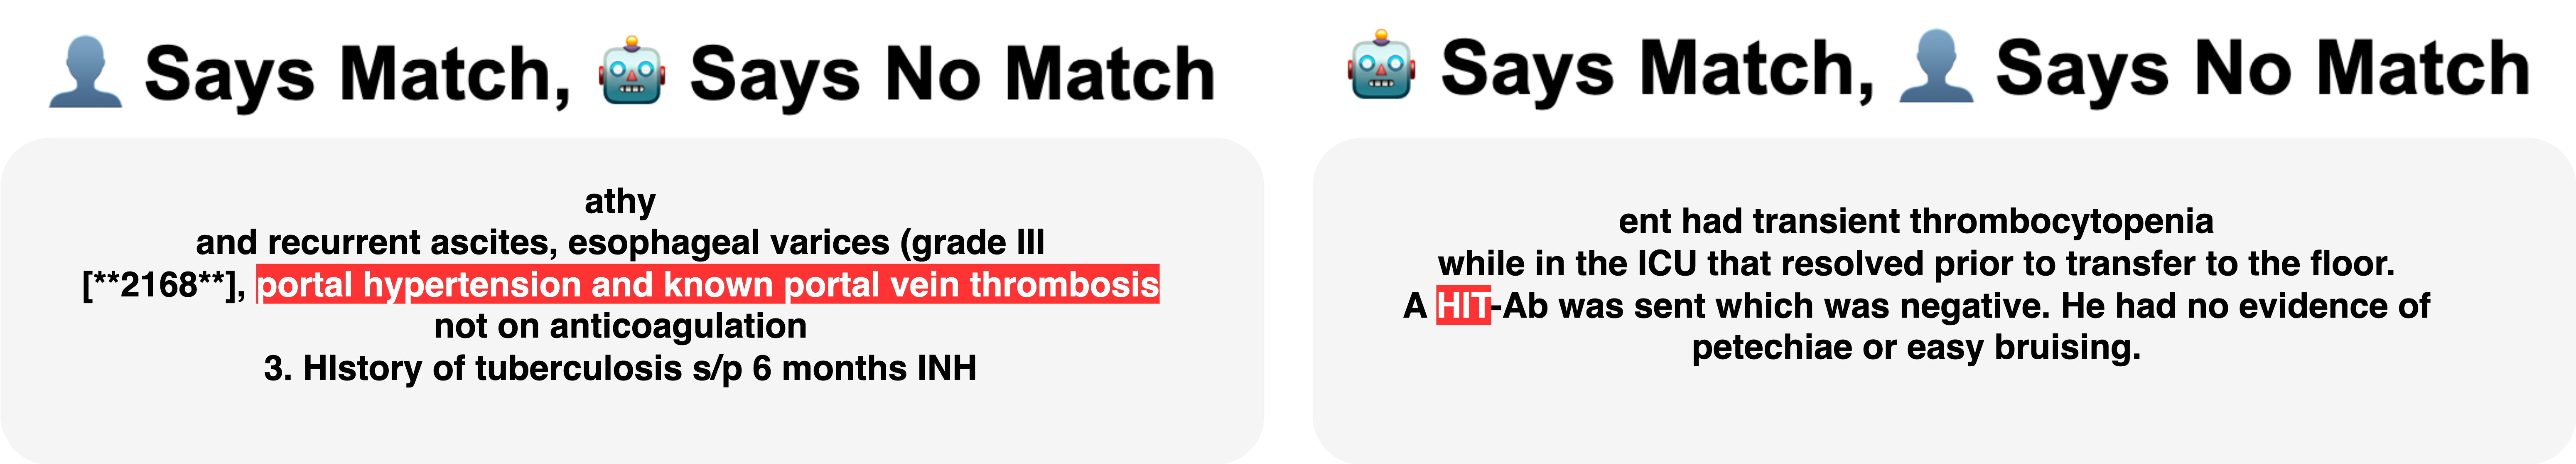
\includegraphics[width=0.8\textwidth]{figs/DisagreementSupervisorVHuman.drawio.png}
    \caption{\textbf{Failure Modes of RDMA in Rare Disease Mining.} When reviewing existing annotations, we showcase two cases where our human annotator disagrees with RDMA's refinement step. Specifically, we see that our refinement agent fails to classify portal vein thrombosis as a rare disease, primarily because its Orphanet listing ``Non-cirrhotic and non-tumoral portal vein thrombosis" does not exactly match the entity ``portal vein thrombosis". On the other hand, while the agent is able to classify ``HIT" as ``heparin induced thrombocytopenia", it does not capture the context "which was negative" properly.}
    \label{fig:annotator_agreement_qualitative}
\end{figure}

\textbf{Examples of RDMA Flagged Entities in Dataset Refinement.} \label{appendix: dataset refinement}
We investigate which entities were primarily flagged by RDMA for human review. We visualize the top cases in Fig. \ref{fig:Top_Corrections}, where we observe that many entities mined by \cite{dong2023ontology_poor_annotations} were indeed not rare diseases, while several key rare disease entities were missed in their original annotations.

\begin{figure}[h!]
    \centering
    \includegraphics[width=1.0\textwidth]{figs/RDMA_Corrections.drawio.png}
    \caption{\textbf{Top 5 Corrected Annotations with RDMA.} RDMA effectively assists human annotation by identifying errors in the noisy historical dataset from \cite{dong2023ontology_poor_annotations}. The figure highlights the top 5 corrections, including both false negatives (a) such as seizure disorder incorrectly labeled as a rare disease in Orphanet, and false positives (b) that were missed in the initial annotations. Of the 72 annotations flagged by RDMA for human review, 55 (76.4\%) were correctly identified as erroneous, demonstrating its value as an annotation assistant for prioritizing human supervision. While hemochromatosis is typically considered a rare condition, in ICU contexts such as MIMIC notes, our physician deemed that to not necessarily be the case. Furthermore, Orphanet \cite{weinreich2008orphanet} makes a distinction between \textbf{rare} hemochromatosis and hemochromatosis. }
    \label{fig:Top_Corrections}
\end{figure}

\clearpage